\section{Unmanned Aircraft}\label{sec:drone}

The unmanned aircraft, UA, commonly called drone, is a vehicle, that to be piloted, doesn't need a person inside of it. Thus, it is necessary to have a system which is able to control the UA in order to accomplish the desired task. This system gives parcial or total automony to the aircraft, meaning that it can be, respectively, a remote control from an operator or onboard computers prepared to act depending on different situations. The remote control from an operator can be either on the ground, in a GS, either in the air, in another vehicles.

Nowadays, the use of UAs is increasing due to the various tasks that they can perform, as surveillance, mapping, aerial photography, monitoring and military applications.

In this project, the operator will be on the ground and the UA will be controlled by a couple of tracking antennas. One antenna will be onboard the aircraft and the other will be on the ground on a base station which will receive and send information from and to the aircraft. 

For this project, eBee will be used as an example and can be observed in Figure \ref{fig:ebee}. This drone was developed by the company senseFly and has three different models: eBee, the mapping drone, eBee RTK, the survey-grade mapping drone and eBee Ag, the precision agriculture drone. Each model was created for a specific task, however the main characteristics are common to every model. The weight of this aircraft varies between 0.69 Kg and 0.73 Kg, the wingspan is 96 cm and they are made of EPP foam and carbon. They are equipped with a 11,1 V battery, which allows a flight time between 40 and 50 minutes, and with a WX camera (18.2 MP) which can be changed by another cameras like the thermoMAP. The thermoMAP captures thermal videos and still images which allows the creation of a full thermal map of a site. The Ground Sampling Distance (GSD), that is the distance measured on the ground between the center of two consecutive pixels when the picture was taken from the air, varies between 1.5 cm and 2 cm (maximum values). 
 
\begin{figure}[H]
  \centering
  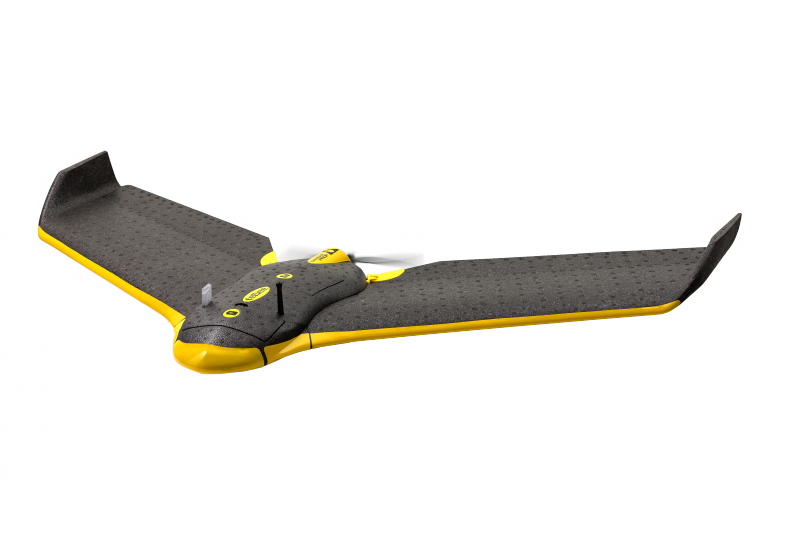
\includegraphics[scale=0.45]{figures/eBee.png}
  %\caption[The professional mapping drone eBee]
   %{The professional mapping drone \textit{eBee} \href{https://www.sensefly.com/drones/ebee.html}{(www.sensefly.com)}. Fully autonomous drone to capture high-resolution aerial photos that can transform into accurate 2D orthomosaics \& 3D models.}
   \caption{Comercial Drone \textit{eBee} \cite{eBee}.}
   \label{fig:ebee}
\end{figure}

The accuracy related to the position depends on the existance of ground control points (GCP). In the table \ref{accuracy} the vertical and horizontal accuracies for each model are described.

\begin{table}[h!]
	\centerline{
	\begin{tabular}{|c||c|c|c|}
		\hline
		Parameter & eBee & eBee RTK & eBee Ag\\ \hline\hline
		Horizontal Accuracy (with GCPs) & Down to 3 cm & - & Down to 4 cm\\ \hline
		Vertical Accuracy (with GCPs) & Down to 5 cm & - & Down to 7 cm\\ \hline
		Horizontal Accuracy (without GCPs) & 1-5 m & Down to 3 cm & 1-5 m\\ \hline
		Vertical Accuracy (without GCPs) & 1-5 m & Down to 5 cm & 1-5 m\\ \hline
	\end{tabular}}
	\caption{GPC Accuracy of the eBee models.}
	\label{accuracy}
\end{table}

The software that is responsible for controlling and planning the flight is called eMotion. This is a GS software and is supplied with every eBee model.